\documentclass[11pt,a4paper,english]{uvamath}
\usepackage[english]{babel}

\usepackage{amsmath, amsfonts, amssymb, a4wide, fancyhdr, lineno, graphicx, epsfig, soul, color, hyperref}
\usepackage[square, numbers]{natbib}

% Running line numbers:
\linenumbers
% Number only every 5:th line:
\modulolinenumbers[5]

%Nodig om een bibliography midden in het artikel te zetten, ipv aan het einde zoals eigenlijk gebruikelijk is
\renewcommand{\bibsection}{}

% TODO command
\newcommand{\todo}[1]{
    \hl{#1}
}

% The things that should be filled in by each group, depending on their situation, are written in a todo command, \todo{like this text}. All text in normal the normal font, is applicable for any group. However, everyone is free to adapt any text, and it is even suggested to look at all text critically and make changes if needed.

% Project specific commands
\author{Tom van Duist \& Kevin van den Bekerom}

\newcommand{\projectname}{\todo{Project Name}\ }


\newcommand{\aanpassen}[1]{ {\sethlcolor{green} \hl{#1}} }

\title{Co-creation workshop}
%Variables
\newcommand{\TitelAbbr}{}
\newcommand{\Version}{0.1}



\what{}
\supervisors{}
\author{Kevin van den Bekerom \& Tom van Duist}


\begin{document}

\maketitle

\clearpage


\chapter{Co-creation workshop planning}
To goal of the Co-creation workshop (CCW) is to come up with methods to raise the Software Engineering course's \textit{quality}.
We measure \textit{quality} by student's final grade for the course, under the assumption that the exercises remain equally difficult. The CCW will be held during the weekly sessions on Thursday, with our colleagues. \\

\section{CCW outline}
We will base the CCW on one iteration of the Nonaka spiral model \cite{nonaka}. In short, we start with a Nominal Group Technique brainstorming session \cite{NGT}. All individual ideas are gathered using a Round Robin protocol. In the second phase we try forming analogous to the suggested ideas. In the third stage we try to group ideas together in logical units. After the third stage comes \textit{internalization}, see figure \ref{fig:spiral}. We will not focus on this stage in the workshop, since it is not feasible withing the allocated time.

\begin{figure}[h]
	\centering
	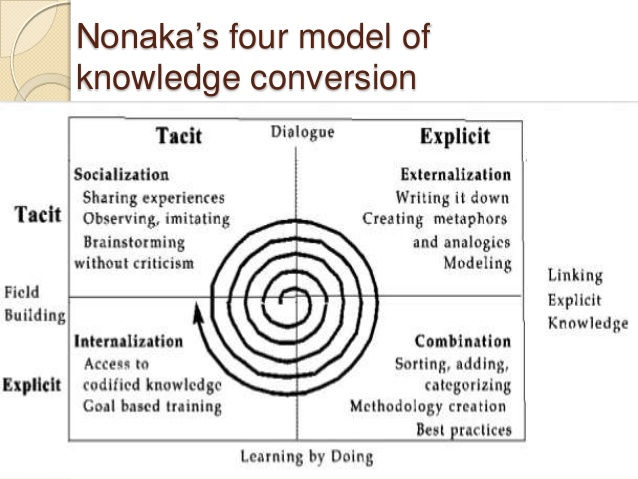
\includegraphics[width=0.75\linewidth]{spiral.jpg}
	\caption{Nanoka's four model of knowledge conversion.}
	\label{fig:spiral}
\end{figure}  

\section{Brainstorming session}
All participants get 5 minutes to write down any ideas they have to meet the CCW's goal. It is stressed - beforehand - that idea's will not be criticized in this stage. Ideas are written down on post-it notes. After the 5 minutes each member delivers their ideas, one idea at a time, in Round Robin fashion. Ideas will NOT be criticized. Questions to clarify the idea are allowed, and should be asked! After the idea is conceptually clear to everyone the group will add one or more keywords to the idea, and places the idea on the wall / whiteboard. This stage ends when all ideas are processed. Real idea discussion comes in the next stage, so the total time of the first stage is set at 10 minutes.

\section{Make analogies}
In this stage we start by rating the ideas on the board, anonymously. The most rated idea gets the higher rank, second most rated second rank, and so forth. Multiple ideas can share the same rank. 

In order of highest to lowest priority ideas will be transformed into analogies that group members are comfortable with. Analogies are hard to make, and caters creativity. New ideas might result from this process. The mental model of each team member will also be aligned, after their is a common analogy.    

\section{Combination}
In this phase ideas are combined, aggregated into groups, as to reveal important aspects. If we can name these concepts we can do further research focusing on those concepts. Aggregation can be based on defined keywords. Common ideas between post-its with different keywords should also be explored.

\chapter{References}

\begin{thebibliography}{9}
	
	\bibitem{nonaka}
	Nonaka, Ikuijiro (1992),
	\textit{The Knowledge-Creating Company}
	Harvard Business Review, 69(November-December, 96-104
	
	\bibitem{NGT}
	Sample, J. A. (1984),
	\textit{Nominal Group Technique: An Alternative to Brainstorming.},
	Journal of Extension, 22 (2). Retrieved November 13,
	2015, from http://www.joe.org/joe/1984march/index.html.
	
	
	
\end{thebibliography}


\appendix


\end{document}
